\chapter{Logistic Regression}
\label{chp:02}

\section{Giới thiệu về Logistic Regression}
\textit{Logistic Regression} là mô hình được đặt tên dựa trên hàm số mà nó đóng vai trò cốt lõi của mô hình, đó là hàm \textit{logistic}. Hàm \textit{logistic} được tạo ra ra bởi những nhà thống kê để đặc tả sự bùng nổ dân số. Hàm \textit{logistic} có dạng hình chữ S có thể nhận đầu vào là số thực và có miền giá trị là $(0, L)$. Biểu thức toán học tổng quát của hàm \textit{logistic}:
%\begin{equation*}
  %f(x)=\frac{L}{1 + e^{-k(x-x_{0})}}
%\end{equation*}
\begin{align*}
f(x)=\frac{L}{1 + e^{-k(x-x_{0})}}, \text{ với} \quad &x_{0} \text{ là giá trị chính giữa của đường cong logistic.}\\
     &k \text{ là tỷ lệ tăng của hàm logistic.}\\
    &L \text{ là giá trị cực đại của hàm logistic.}
\end{align*}

Mô hình \textit{Logistic Regression} giống \textit{Linear Regression} ở khía cạnh sử dụng biểu thức toán học để biển diễn, và giống với \textit{Perception Learning Algorithm} ở việc đầu ra bị chặn. Tuy nhiên, \textit{Logistic Regression} thường được sử dụng nhiều hơn cho các bài toán phân loại mặc dù trong tên có chứa từ $"Regression"$. Trong phần tiếp theo sẽ làm rõ tại sao \textit{Logistic Regression} lại thích hợp với bài toán phân loại, đặc biệt là phân loại nhị phân.

\section{Bài toán Supervised learning và hàm Sigmoid activation}
Cũng giống như \textit{Linear Regression}, \textit{Logistic Regression} được sử dụng để giải bài toán \textit{Supervised Learning}. Tuy nhiên, \textit{Logistic Regression} được dùng để giải các bài toán phân loại, còn \textit{Linear Regression} được dùng để dự đoán cho các bài toán có giá trị liên tục (như dự đoán giá nhà). Câu hỏi đặt ra là tại sao không dùng \textit{Linear Regression} thay vì \textit{Logistic Regression} để giải bài toán phân loại. Chúng ta sẽ lấy ví dụ để minh chứng sự vượt trội của \textit{Logistic Regression} so với \textit{Linear Regression} khi áp dụng vào bài toán phân loại, cụ thể là phân loại nhị phân.
\\
\begin{exmp}
\label{exmp:o}
\hrulefill\\
%%%
Một nhóm 20 người có chiều cao từ 1.4 m đến 1.8 m. Từ chiều cao của mỗi người chúng ta sẽ dự đoán xem họ là nam (M) hay nữ (F).\\
\\
Ta có tập dữ liệu như bảng \ref{Tab:ex}:\\
\begin{table*}[ht]
\centering
\begin{tabular}{|l|l|l|l|}
\hline
Height & Gender \\ \hline
1.5   & F \\ \hline
1.75  & M \\ \hline
1.6     & M \\ \hline
1.45  & F  \\ \hline
1.55   & F \\ \hline
1.7  & M \\ \hline
1.65  & M \\ \hline
1.4     & F \\ \hline
1.8  & M \\ \hline
1.6.5   & M \\ \hline
1.65  & F \\ \hline
1.55   & M \\ \hline
1.6  & F \\ \hline
1.5   & M \\ \hline
\end{tabular}
\caption{Dữ liệu đầu vào của ví dụ \ref{exmp:o}}
\label{Tab:ex}
\end{table*}
\end{exmp}

Để trực quan hơn, ta biểu diễn dữ liệu trên tọa độ không gian 2 chiều ở hình \ref{fig:sec2ex1}:
\begin{figure}[!ht]
    \centering
    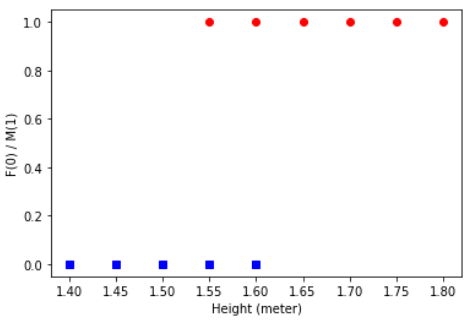
\includegraphics[scale=0.5]{books/artificial-neural-network/chapter02/figure/example1.png}
    \caption{Đồ thị các điểm dữ liệu.}
    \label{fig:sec2ex1}
\end{figure}

Trong ví dụ này, đầu vào của mô hình là vector $\mathbf{X}$ tương ứng với chiều cao của nhóm người và đầu ra là vector $\mathbf{y}$ tương ứng với giới tính của họ (M/F). Ta khởi tạo vector trọng số $\mathbf{W}$ có chiều dài bằng với vector $\mathbf{X}$ và biến $\mathbf{b}$ (bias). Gọi $\mathbf{\hat{y}}$ là xác suất một người là nam khi biết chiều cao của người đó là ($\hat{y}$ $=$ $P(y=1|x)$) và $\mathbf{\hat{y}}$ nằm trong khoảng $[0, 1]$.

%Tiếp theo, ta làm rõ tại sao \textit{Linear Regression} không phù hợp với bài toán phân loại.\\

Trong mô hình \textit{Linear Regression}, ta có đầu ra dự đoán là:
\begin{equation*}
    \hat{y} = z = W^TX + b
\end{equation*}

Khi áp dụng \textit{Linear Regression} vào bài toán trên chúng ta có thể thu được kết quả như hình \ref{fig:lr_result}:
\clearpage
\begin{figure}[!ht]
    \centering
    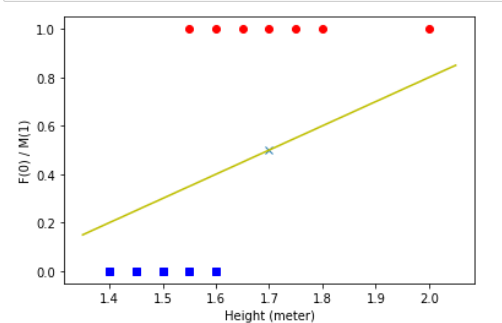
\includegraphics[width=\textwidth,height=\textheight,keepaspectratio]{books/artificial-neural-network/chapter02/figure/LN_result.PNG}
    \caption{Kết quả khi dùng Linear Regression.}
    \label{fig:lr_result}
\end{figure}

Trong hình \ref{fig:lr_result}, đường màu vàng biểu diễn đường \textit{Linear Regression}. Có hai vấn đề có thể thấy được từ kết quả của \textit{Linear Regression}:

\begin{itemize}
    \item Đường thẳng \textit{Linear Regression} không bị chặn nên nó thể cho ra kết quả không nằm trong vùng mong muốn như trên hình trên đường thẳng có thể cho ra giá trị $\mathbf{\hat{y}}$ > 1 và $\mathbf{\hat{y}}$ < 0 nên mô hình này không phù hợp cho bài toán này. Tuy nhiên, chúng ta có thể chặn đường thẳng trên bằng cách cắt phần nhỏ hơn 0 bằng cách cho chúng bằng 0, cắt các phần lớn hơn 1 bằng cách cho chúng bằng 1.
    \item \textit{Linear Regression} không có khả năng phân loại tốt với dự liệu bị mất cân bằng. Nếu chúng ta lấy điểm trên đường thẳng này có tung độ bằng 0.5 là điểm ngưỡng phân chia hai lớp (là nam nếu $\mathbf{\hat{y}}$ $> 0.5$, ngược lại là nữ). Giả sử có thêm một người có chiều cao 1.9 mét và là nam. Khi áp dụng mô hình \textit{Linear Regression}, đường thẳng sẽ bị lệch về bên phải (như hình \ref{fig:lr_result}) sẽ dẫn đến hiện tượng toàn bộ những người nữ vẫn được dự đoán là nữ, nhưng những người là nam nhưng được dự đoán là nữ.
\end{itemize}

Vì vậy chúng ta cần một mô hình khác thể cho ta đường phân chia tốt hơn so với \textit{Linear Regression} và thỏa mãn các tính sau:

\begin{itemize}
    \itemsep0em
    \item Là hàm số nhận giá trị thực, bị chặn trong khoảng (0,1).
    \item Nếu coi điểm có tung độ là $0.5$ làm điểm phân chia thì các điểm càng xa điểm này về phía bên trái có giá trị càng gần $0$. Ngược lại, các điểm càng xa điểm này về phía phải có giá trị càng gần 1. Điều này khớp với nhận xét rằng học càng nhiều thì xác suất đỗ càng cao và ngược lại.
    \item Hàm liên tục để có thể đạo hàm mọi nơi, để giúp tìm điểm tối ưu khi sử dụng \textit{Gradient Descent}.
\end{itemize}

Ta thấy, Hàm \textit{Sigmoid} (là hàm \textit{Logistic} với $L = 1$, $k = 1$ và $x_{0} = 0$) thỏa mãn 3 tính chất nói trên. Phương trình của hàm \textit{Sigmoid}:

\begin{equation}
    f(z)= \sigma(z) = \frac{1}{1 + e^{-z}}
    \label{eq:esigmoid}
\end{equation}

Đồ thị của hàm \textit{Sigmoid}:
\begin{figure}[!ht]
    \centering
    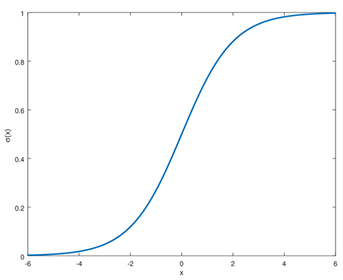
\includegraphics[scale=0.8]{books/artificial-neural-network/chapter02/figure/sigmoid.png}
    \caption{Đồ thị các điểm dữ liệu.}
    \label{fig:sigmoid}
\end{figure}

Từ phương trình (\ref{eq:esigmoid}) và đồ thị hình \ref{fig:sigmoid}, ta có thể dễ dàng thấy \newline $\lim_{s \rightarrow -\infty}\sigma(s) = 0$ và $\lim_{s \rightarrow +\infty}\sigma(s) = 1$. Vì vậy miền giá trị của hàm \textit{Sigmoid} luôn là $(0, 1)$, rất thích hợp với việc phân loại nhị phân. Ngoài ra, khi đầu vào  rất lớn (hoặc rất nhỏ) thì giá trị đầu ra của hàm \textit{Sigmoid} luôn tiến tới tiệm cận 1 hoặc 0, nên hàm \textit{Sigmoid} có thể xử lý việc dữ liệu bị mất cân bằng, là vấn đề đã nêu trên của \textit{Linear Regression}. Áp dụng hàm \textit{Sigmoid} vào ví dụ \ref{exmp:o}, ta lấy $\mathbf{W^TX + b}$ làm dữ liệu đầu vào của hàm \textit{Sigmoid}. Phương trình mới của kết quả dự đoán $\hat{y}$:
\begin{align*}
    \hat{y}= \sigma(z) = \sigma(W^TX + b)
\end{align*}

%\end{equation*}
Với ngưỡng phân loại là 0.5, như  kết quả thu được ở hình \ref{fig:lg_result}: ta có thể thấy, \textit{Logistic Regression} có khả năng phân loại tốt hơn nhiều so với \textit{Linear Regression},

\begin{figure}[!ht]
    \centering
    %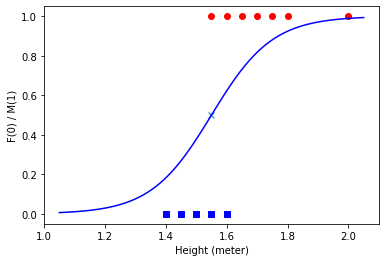
\includegraphics[width=\textwidth,height=\textheight,keepaspectratio]{books/artificial-neural-network/chapter02/figure/LG_result.png}
    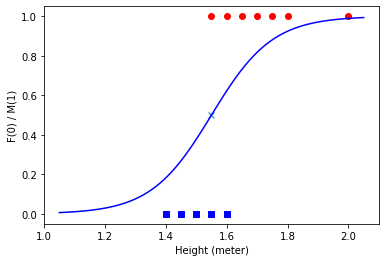
\includegraphics[scale=0.8]{books/artificial-neural-network/chapter02/figure/LG_result.png}
    \caption{Kết quả khi dùng Logistic Regression.}
    \label{fig:lg_result}
\end{figure}

\section{Hàm Cost function của Logistic Regression}
Trước khi đi vào nội dung chính của phần này, chúng ta sẽ tìm hiểu về khái niệm hàm lồi (convex function) và hàm không lồi (non-convex function):

\begin{itemize}
    \item Hàm $f$ được gọi là lồi trên đoạn $[\alpha, \beta] \subset R$ nếu với mọi $x,y \in [\alpha, \beta]$ và với mọi $a, b \geq 0$ thỏa $a + b = 1$ thì: $f(ax + by) \geq af(x) + bf(y)$. Nếu $f$ là hàm lồi trên $[\alpha, \beta]$ thì ta có: $min(f)=min{f(\alpha), f(\beta)}$ nên hàm lồi chỉ có 1 điểm cực tiểu và đó là điểm mà hàm có giá trị nhỏ nhất trên miền giá trị của nó (global minimum).
    \item Hàm $f$ được gọi là hàm không lồi khi nó không có tính chất lồi. Đồ thị hàm không lồi thường có dạng sóng với nhiều điểm cực trị (cực tiểu hoặc cực đại) (local optimal).
\end{itemize}

\begin{figure}[!htb]
   \begin{minipage}{0.48\textwidth}
     \centering
     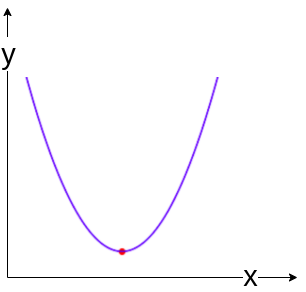
\includegraphics[width=1\linewidth]{books/artificial-neural-network/chapter02/figure/convex.png}
   \end{minipage}\hfill
   \begin{minipage}{0.48\textwidth}
     \centering
     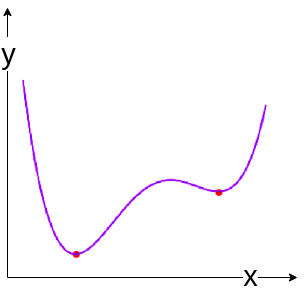
\includegraphics[width=1\linewidth]{books/artificial-neural-network/chapter02/figure/non_convex.png}
   \end{minipage}
   \caption{Đồ thị hàm convex (bên trái) và đồ thị hàm non-convex (bên phải)}
   \label{fig:convex}
\end{figure}

Tiếp theo ta sẽ đi vào nội dung chính của phần này. Nhắc lại, trong mô hình \textit{Logistic Regression}, ta có:
\begin{equation*}
    \hat{y}= \sigma(z) = \sigma(W^TX + b)
\end{equation*}

Cũng như phương pháp giải các bài toán \textit{Supervised Learning}, quá trình học của mô hình \textit{Logistic Regression} là quá trình cập nhật trọng số $\mathbf{W}$ vì vậy \textit{Logistic Regression} cũng cần có một hàm mất mát (Loss Function) để đánh giá sự sai biệt giữa kết quả dự đoán $\hat{y}$ và kết quả thực tế $y$. Ta ký hiệu $\mathcal{L}(\hat{y}, y)$ là hàm mất mát.

Hàm mất mát đơn giản nhất chính là \textit{Least Squared Error (LSE)} có phương trình là:
\begin{equation*}
    \mathcal{L}(\hat{y}, y) = \frac{1}{2}(\hat{y} - y)^2
\end{equation*}

%Vì phương trình kết quả dự đoán của \textit{Linear Regression} là $\hat{y} =  w^TX + b$ nên hàm LSE là hàm lồi và chúng ta có thể đạt được điểm tối ưu của hàm với giá trị mất mát nhỏ nhất (hình 1.5 bên trái).
Tuy nhiên, đối với \textit{Logistic Regression}, chúng ta không dùng LSE làm hàm mất mát bởi vì phương trình kết quả dự đoán của \textit{Logistic Regression} $\hat{y} = \sigma(w^TX + b)$ nên khi đó LSE là một hàm không lồi với nhiều điểm cực tiểu (hình \ref{fig:convex} bên phải).

LSE không đảm bảo tìm được điểm tối ưu toàn cục khi giải bài toán \textit{Logistic Regression}. Vì vậy, chúng ta cần có một hàm mất mát khác cho \textit{Logistic Regression} và đó là hàm \textit{Cross-Entropy}. Phương trình hàm mất mát khi đó:
\begin{equation} \label{eq:ce}
    \mathcal{L}(\hat{y}, y) = -(y\log_{}{\hat{y}} + (1 - y)\log_{}{(1 - \hat{y})})
\end{equation}

Vì tập giá trị của $y$ là $\{0,1\}$ nên từ phương trình \eqref{eq:ce}, ta có thể thấy:
\begin{itemize}
    \item Khi $y = 0$: phương trình \eqref{eq:ce} sẽ trở thành $L(\hat{y}, y) = -\log_{}{(1 - \hat{y})}$. Trong trường hợp này, nếu kết quả dự đoán $\hat{y}$ của chúng ta càng gần về giá trị $0$ thì hàm mất mát cho ra giá trị càng nhỏ và ngược lại, đáp ứng đúng như yêu cầu chúng ta mong muốn.
    \item  Khi $y = 1$: phương trình \eqref{eq:ce} sẽ trở thành $L(\hat{y}, y) = -\log_{}{(\hat{y})}$. Trong trường hợp này, nếu kết quả dự đoán $\hat{y}$ của chúng ta càng gần về giá trị $1$ thì hàm mất mát cho ra giá trị càng nhỏ và ngược lại, đáp ứng đúng như yêu cầu chúng ta mong muốn.
    \item Với việc $\hat{y}$ bằng các giá trị đầu mút ($0$ và $1$) khi và chỉ khi đầu vào của hàm sigmoid là vô cùng, điều không xảy ra với các phép toán tự nhiên nên ta có thể thấy hàm mất mát luôn cho giá trị có ý nghĩa.
\end{itemize}

Tiếp theo, chúng ta sẽ giải thích tại sao \textit{Cross-Entropy} có thể giúp mô hình \textit{Logistic Regression} tìm được điểm tối ưu toàn cục. Để dễ dàng chứng minh ta viết lại phương trình của kết quả dự đoán $\hat{y}$ như sau:
\begin{equation*}
    \hat{y} = \theta^TX
\end{equation*}
\begin{align*}
  \text{với} \quad &X \text{ là ma trận đầu vào có thêm một cột vector có giá trị của các hàng }\\
  & \text{đều bằng 1 (giá trị của bias)}\\
     &\theta \text{ là các trọng số của mô hình Logistic Regression.}
\end{align*}
Từ phương trình \eqref{eq:ce}, ta có:
%\begin{equation*}
\begin{align}
-\mathcal{L}(\hat{y}, y) & = y\log_{}{\hat{y}} + (1 - y)\log_{}{(1 - \hat{y})} \nonumber\\
              & = y\log_{}{(\frac{1}{1 + e^{-\theta^TX}})} + (1 - y)\log_{}{(1 - \frac{1}{1 + e^{-\theta^TX}})} \nonumber\\
              & = y\log_{}{(\frac{e^{\theta^TX}}{1 + e^{\theta^TX}})} + (1 - y)\log_{}{(\frac{1}{1 + e^{\theta^TX}})} \nonumber\\
              & = y\log_{}{(e^{\theta^TX})} - y\log_{}{(1+ e^{\theta^TX})} + (1 - y)\log_{}{(1)} + (1 - y)\log_{}{(1 + e^{\theta^TX})} \nonumber\\
-\mathcal{L}(\hat{y}, y) & = y\theta^TX - \log_{}{(1 + e^{\theta^TX})} \nonumber\\
f(X) = \mathcal{L}(\hat{y}, y) & = \log_{}{(1 + e^{\theta^TX})} - y\theta^TX \nonumber\\
\frac{\partial f}{\partial \theta} & = \frac{1}{1 + e^{-\theta^TX}}Xe^{\theta^TX} - Xy \nonumber\\
%\begin{align}
\label{eqn:n1} & = \frac{X}{1 + e^{\theta^TX}} - Xy  \\
\label{eqn:n2} \frac{\partial^2 f}{\partial \theta^2} & = -\frac{X^2}{1 + e^{\theta^TX}}
\end{align}
%\end{equation*}

Từ (\ref{eqn:n1}) ta có thấy $f$ có một điểm cực trị là $\theta^T = \ln{(y^{-1} - 1)}X^{-1}$. Và từ (\ref{eqn:n2}) ta thấy đạo hàm cấp 2 của $f$ theo $\theta$ luôn âm nên điểm cực trị này là điểm cực tiểu toàn cục (global minimum) của hàm $f$. Từ đó, có thể thấy ta có thể tìm được điểm tối ưu toàn cục của mô hình \textit{Logistic Regression} khi sử dụng hàm \textit{Cross-Entropy} làm hàm mất mát.

Phương trình (\ref{eq:ce}) là hàm mất mát của một điểm dữ liệu đầu vào (Loss Function). Vậy với tập dữ liệu đầu vào có kích thước là $m$ chúng ta sẽ có được phương trình tổng quát của hàm mất mát (Cost Function) trong mô hình \textit{Logistic Regression} như phương trình (\ref{eq:cf}):
\begin{equation}
    J(W, b) = \frac{1}{m}\sum_{i = 1}^m\mathcal{L}(\hat{y}^{(i)}, y^{(i)})
    \label{eq:cf}
\end{equation}

\section{Sử dụng gradient descent để tìm giá trị tối ưu}
Nhắc lại về hàm \textit{cost function} của \textit{logistic regression}:
\begin{center}
$J(w, b) = \frac{-1}{m}\sum_{i=1}^{m}y^{(i)}\log \hat{y}^{(i)}+(1-y^{(i)})\log (1-\hat{y}^{(i)})$
\end{center}
Với:
\begin{center}
$\hat{y}=\sigma (w^{T}x + b)$\\
$\sigma (z) = \frac{1}{1+e^{-z}}$\\
\end{center}

Hàm \textit{cost function} này cho ta biết được mức độ sai khác giữa giá trị đầu ra ta tính được từ dữ liệu đầu vào ($\hat{y}$) và giá trị đầu ra thật sự của dữ liệu ($y$) dựa trên giá trị của $w$ và $b$. Vì vậy, nếu giá trị của \textit{cost function} càng nhỏ, thì dữ liệu mà ta tính toán được sẽ càng giống với dữ liệu thật sự. Bài toán bây giờ của chúng ta chính là tìm giá trị của $w$ và $b$ sao cho giá trị của \textit{cost function}là nhỏ nhất.

\textit{Gradient decent} là một phương pháp được sử dụng rộng rãi để tìm kiếm giá trị tối ưu của \textit{cost function}. Với một hàm khả vi và là hàm lồi, ta có thể sử dụng \textit{gradient decent} để tìm được giá trị gần tối ưu của hàm đó.

Để hiểu rõ hơn về \textit{gradient decent}, ta sẽ lấy một ví dụ đơn giản về việc sử dụng phương pháp này để tìm giá trị tối ưu của hàm số.
\clearpage
\begin{figure}[!h]
\centerline{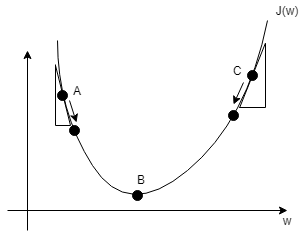
\includegraphics{books/artificial-neural-network/chapter02/figure/grad_1.png}}
\caption{Đồ thị minh hoạ \textit{gradient decent}.}
\label{fig:grad_1}
\end{figure}

Hình trên là một đồ thị biểu diễn hàm số $J(w)$ có B là điểm tối ưu. Để đến được vị trí B, đầu tiên ta sẽ chọn một điểm bất kì thuộc đồ thị. Sau đó, ta thay đổi vị trí của điểm đó dựa trên giá trị đạo hàm. Việc cập nhật sẽ được lặp lại cho đến khi điểm ta chọn chạy đến vị trí B. Khi đó, ta đã tìm được giá trị tối ưu của hàm $J(w)$

Công thức của \textit{gradient decent} là:
\begin{center}
$w = w - \alpha\frac{\delta J(w)}{\delta w}$
\end{center}

Với $\alpha$ được gọi là \textit{learning rate}, dùng để xác định độ dài bước đi mỗi lần cập nhật và giá trị $\alpha$ luôn lớn hơn $0$.

Nếu ta lấy điểm khởi đầu là A, thì khi đó, đạo hàm tại điểm A sẽ là âm (do $\Delta J(w_{A})$ âm còn $\Delta w_{A}$ dương). Giá trị $w$ được cập nhật sẽ tăng lên (do $-\alpha\frac{\delta J(w_{A})}{\delta w_{A}} > 0$). Ta có thể thấy điểm A sẽ dời về phía bên phải và di chuyển gần hơn đến giá trị tối ưu B.

Trường hợp khác, nếu ta lấy điểm bắt đầu là điểm C, đạo hàm tại điểm C sẽ có giá trị là dương (do $\Delta J(w_{C})$ dương và $\Delta w_{C}$ dương). Giá trị $w$ sẽ giảm xuống (do $-\alpha\frac{\delta J(w_{A})}{\delta w_{A}} < 0$). Điều đó làm cho điểm C sẽ di chuyển về phía bên trái và đến gần hơn với giá trị tối ưu B.

Với số lần lặp vừa đủ và chọn giá trị \textit{learning rate} vừa phải, từ 1 điểm bất kì được chọn trên hàm số, ta đều có thể di chuyển về điểm tối ưu của hàm số.

\begin{figure}[!h]
\centerline{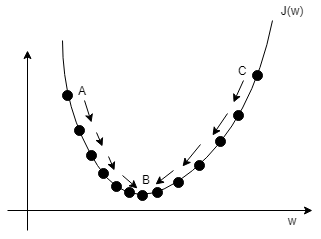
\includegraphics{books/artificial-neural-network/chapter02/figure/grad_2.png}}
\caption{Kết quả khi sử dụng \textit{gradient decent} để tìm giá trị tối ưu}
\label{fig:grad_2}
\end{figure}

Ta có thể thấy, khi sử dụng \textit{gradient decent}, ta sẽ về được giá trị tối ưu của hàm số dù điểm khởi đầu của ta có thể nằm ở vị trí vào. Như hình \ref{fig:grad_2}, từ điểm A hay C của đồ thị, với số lần lặp vừa đủ và \textit{learning rate} vừa phải, ta sẽ chạy được về điểm tối ưu B của hàm số.

Để sử dụng \textit{gradient decent} tìm giá trị tối ưu, ta phải lựa chọn \textit{learning rate} $\alpha$ không quá lớn hay quá nhỏ. Nếu lựa chọn giá trị $\alpha$ quá lớn, quá trình lặp khi sử dụng \textit{gradient decent} sẽ không chạy về giá trị tối ưu nữa mà sẽ hạy ra xa điểm tối ưu. Còn nếu giá trị $\alpha$ quá nhỏ, số lần lặp để tới được điểm tối ưu sẽ lớn hơn nhiều. Điều này làm cho thời gian chạy để tìm được điểm tối ưu sẽ lâu hơn rất rất nhiều.

\clearpage
\begin{figure}[!htb]
   \begin{minipage}{0.48\textwidth}
     \centering
     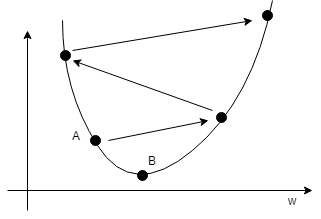
\includegraphics[width=1\linewidth]{books/artificial-neural-network/chapter02/figure/grad_3.png}
   \end{minipage}\hfill
   \begin{minipage}{0.48\textwidth}
     \centering
     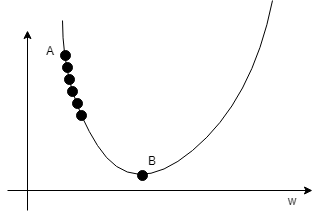
\includegraphics[width=1\linewidth]{books/artificial-neural-network/chapter02/figure/grad_4.png}
   \end{minipage}
   \caption{\textit{gradient decent} khi giá trị $\alpha$ quá lớn (trái) và quá nhỏ (phải).}
\end{figure}

Với hình bên trái, đây là khi ta lựa chọn giá trị $\alpha$ quá lớn. Với điểm khởi đầu là A, tại đây khi tính đạo hàm và cập nhật hướng về phía bên phải là chính xác, nhưng khi ta thiết lập giá trị $\alpha$ quá lớn, giá trị mới cập nhật sẽ không phải gần hơn đến điểm tối ưu mà còn bước vượt qua điểm tối ưu này. Nếu quá trình trên được lặp lại với $\alpha$ quá lớn, thì càng ngày ra sẽ đi ra xa điểm tối ưu và sẽ không tìm được kết quả mong đợi.

Với hình bên phải, đây là khi ta chọn giá trị $\alpha$ quá nhỏ. Với điểm khởi đầu ngẫu nhiên ta chọn là A, ta vẫn di chuyển về vị trí tối ưu nhưng bởi vì giá trị $\alpha$ quá nhỏ, mỗi lần lặp ta chỉ có thể đi về phía tối ưu một khoảng quá ngắn. Vì vậy để về điểm tối ưu, ta phải lặp đi lặp lại quá nhiều bước. Kết quả là thời gian ta đến được điểm cần tìm quá lâu cũng như quá tốn tài nguyên tính toán.

Vì thế, để giải thuật \textit{gradient decent} chạy tốt, ta cần phải lựa chọn giá trị $\alpha$ cho phù hợp để có thể tìm được giá trị tối ưu một cách nhanh nhất và chính xác.

\textit{Gradient decent} cũng chỉ có thể tìm được điểm tối ưu khi hàm số thoả mãn những yêu cầu nhất định. Đó chính là khả vi và phải là hàm lồi. Nếu không thoả mãn 2 yếu tố trên, giải thuật này sẽ không tìm được điểm tối ưu.

Với yếu tố khả vi, ta có thể thấy việc chỉ ra hướng để đi đến điểm tối ưu của \textit{gradient decent} dựa trên giá trị của đạo hàm ($w = w - \alpha\frac{\delta J(w)}{\delta w}$). Nếu hàm số không khả vi, là ta sẽ không thể tính được giá trị $\frac{\delta J(w)}{\delta w}$ cũng như việc tìm được điểm tối ưu là không khả thi.

Với yếu tố hàm số phải là hàm lồi, đây là yếu tố quan trọng để xác định xem ta có thể tìm được điểm tối ưu của hàm số hay không. Vì nếu không là hàm lồi, tuỳ thuộc vào vị trí khởi tạo mà giá trị tối ưu ta thu được sau khi sử dụng \textit{gradient decent} có thể là điểm tối ưu cục bộ, không phải điểm tối ưu toàn cục.

\begin{figure}[!h]
\centerline{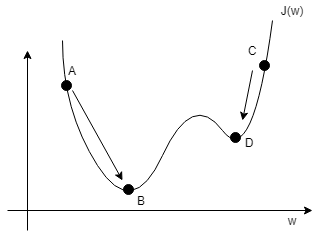
\includegraphics{books/artificial-neural-network/chapter02/figure/grad_5.png}}
\caption{Sử dụng \textit{
gradient decent} không hàm số không là hàm lồi}
\label{fig:grad_5}
\end{figure}

Đồ thị trên là đồ thị của một hàm không là hàm lồi. Những hàm này ngoài điểm tối ưu toàn cục thì còn có các điểm tối ưu cục bộ. Nếu ta lấy điểm khởi đầu là điểm A, thì sau khi sử dụng \textit{gradient decent}, điểm tối ưu ta tìm được vẫn là điểm tối ưu toàn cục là điểm B. Nhưng nếu điểm khởi đầu của chúng ta là điểm C. Khi đó, sau khi dùng \textit{gradient decent} thì điểm tối ưu mà ta tìm được chính là điểm D, và D không là điểm tối ưu cục bộ của hàm. Vì thế, khi sử dụng \textit{gradient decent} với hàm số không là hàm lồi, giá trị tối ưu ta tìm được có thể không là điểm tối ưu toàn cục.

Trên thực tế, khi sử dụng \textit{gradient decent}, ta chỉ có thể tìm được vị trí gần với điểm tối ưu cục bộ.

\clearpage
\begin{figure}[!h]
\centerline{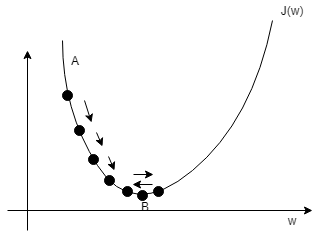
\includegraphics{books/artificial-neural-network/chapter02/figure/grad_6.png}}
\caption{Kết quả của \textit{gradient decent} thực tế}
\label{fig:grad_6}
\end{figure}

Như hình trên, ta lấy điểm khởi đầu là A. Sau đó, sử dụng \textit{gradient decent} để tìm giá trị tối ưu. Khi này, kết quả của chúng ta sẽ chạy lại gần điểm B. Nhưng, khi lại gần B đến một khoảng nhất định, thì khi ta cập nhật giá trị sau khi sử dụng \textit{gradient decent}, kết quả là ta sẽ vượt qua giá trị tối ưu 1 khoảng rất nhỏ. Và khi ta lặp lại \textit{gradient decent} 1 lần nữa, thì ta sẽ đi qua điểm tối ưu 1 khoảng nhỏ tiếp tục. Và cứ như thế, khi chạy \textit{gradient decent}, kết quả mà ta nhận được sẽ dao động môt khoảng nhỏ xung quanh giá trị tối ưu B. Nhưng giá trị sai khác khi ta dùng \textit{gradient decent} và giá trị tối ưu là rất nhỏ. Vì thế, kết quả ta thu được sau khi sử dụng \textit{gradient decent} vẫn rất tốt khi áp dụng vào các bài toán tìm giá trị tối ưu.

Quay trở lại với bài toán tìm giá trị nhỏ nhất của hàm \textit{cost function}, hàm số của chúng ta gồm 2 biến đó chính là $w$ và $b$. Vì thế, mỗi lần lặp của \textit{gradient decent}, ta cần phải cập nhật giá trị của cả $w$ và $b$ bằng cách sử dụng đạo hàm từng phần hàm số với lần lượt 2 biến.

Với \textit{cost function}:
\begin{center}
$J(w, b) = \frac{-1}{m}\sum_{i=1}^{m}y^{(i)}\log \hat{y}^{(i)}+(1-y^{(i)})\log (1-\hat{y}^{(i)})$
\end{center}

Ta sẽ sử dụng đạo hàm từng phần với mỗi biến của \textit{cost function} là $w$ và $b$. Kết quả cập nhật của mỗi biến qua mỗi lần lặp của \textit{gradient decent} là:
\begin{center}
$w = w - \alpha\frac{\delta J(w, b)}{\delta w}$\\
$b = b - \alpha\frac{\delta J(w, b)}{\delta b}$
\end{center}

Ta cập nhật giá trị của $w$ và $b$ với số lần lặp vừa đủ cùng $\alpha$ vừa phải sẽ tìm ra được giá trị tối ưu của hàm \textit{cost function}. Để tính được giá trị của $\frac{\delta J(w, b)}{\delta w}$ và $\frac{\delta J(w, b)}{\delta b}$, ta có thể dùng \textit{computation graph} để tìm được các giá trị đó.

\section{Cách tính đạo hàm riêng dưới góc nhìn Computation graph}
\textit{Computation graph} là một phương pháp giúp tìm đạo hàm riêng một biến của hàm số. Hàm được biểu diễn thành một đồ thị với các đỉnh con là kết quả phép tính của 2 đỉnh cha. Ta sẽ tính giá trị đạo hàm tại mỗi đỉnh của đồ thị bằng cách lấy giá trị xấp xỉ và lan truyền ngược giá trị về đỉnh cha cho đến biến mà ta cần tính đạo hàm. Ta sẽ xem qua ví dụ về việc sử dụng \textit{computation graph} để tính đạo hàm riêng.
\begin{figure}[!h]
\centerline{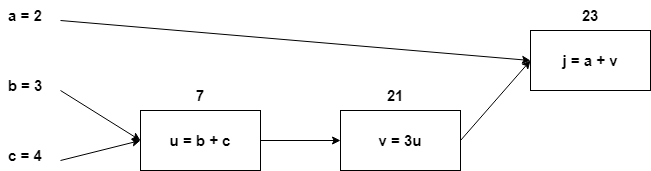
\includegraphics[scale=0.5]{books/artificial-neural-network/chapter02/figure/com_1.png}}
\caption{Ví dụ sử dụng \textit{computation graph} để tính đạo hàm}
\label{fig:com_1}
\end{figure}

Hình trên biểu diễn một hàm số $J$ sử dụng \textit{computation graph}. Hàm số được chia nhỏ thành từng phần và giá trị mỗi phần được tính với các giá trị a, b, c được cho trước. Hàm $J$ có phương trình là:
\begin{equation}
\label{sec2:eqn6}
J = a + 3(b + c)
\end{equation}

Ta chia nhỏ biểu thức \ref{sec2:eqn6} trên bằng các biểu thức nhỏ hơn:
\begin{align}
\label{sec2:eqn7}
u &= b + c\\
\label{sec2:eqn8}
v &= 3u\\
\label{sec2:eqn9}
J &= a + v
\end{align}

Với mỗi biểu thức trên là một đỉnh của đồ thị, ta sẽ được một \textit{computation graph} như hình trên. Tiếp theo, ta sẽ tính đạo hàm tại mỗi đỉnh bằng cách xấp xỉ và lan truyền giá trị ngược lại.

%Với hàm số $f(h(x))$, ta có thể tính đạo hàm của $x$ theo $f$ bằng cách:
%\begin{center}
%$\frac{\delta f}{\delta x} = \frac{\delta f}{\delta h}\frac{\delta h}{\delta x}$
%\end{center}
%Lấy ví dụ ta tính đạo hàm của $a$ theo $J$ tại $a=2$. Dựa vào công thức trên, ta có đạo hàm của $J$ theo $a$ là:
%\begin{center}
%$\frac{\delta J}{\delta a} = \frac{\delta J}{\delta v}\frac{\delta v}{\delta a}$
%\end{center}
Ta sẽ tính đạo hàm tại $a=2$ bằng phương pháp xấp xỉ. Ta chọn $a_{1}$ sao cho $\Delta a$ rất nhỏ ($0.001$). Ta lấy $a_{1} = 2.001$.Từ biểu thức \ref{sec2:eqn9}, suy ra:
\begin{equation}
\label{sec2:eqn10}
J_{1} = a_{1} + v = 23.001
\end{equation}

Ta tính giá trị đạo hàm của $J$ theo $a$ và $J_{1}$ từ \ref{sec2:eqn10}:
\begin{equation}
\label{sec2:eqn11}
\frac{\Delta J}{\Delta a} = \frac{J_{1} - J}{a_{1} - a} = \frac{23.001-23}{2.001-2} = 1\\
\end{equation}

%Sau đó, ta lan truyền kết quả lên để tính đạo hàm của $J$ theo $a$ dựa trên đạo hàm của $J$ theo $v$ và đạo hàm của $v$ theo $a$:
%\begin{center}
%$\frac{\Delta v}{\Delta a} = \frac{v_{1} - v}{a_{1} - a} = \frac{11.001-11}{5.001-5} = 1$\\
%\end{center}
Ta có thể xấp xỉ $\frac{\Delta J}{\Delta a}$ bằng $\frac{\delta J}{\delta a}$. Từ \ref{sec2:eqn11}, giá trị đạo hàm của $J$ tại $a=2$ xấp xỉ:
\begin{center}
$\frac{\Delta J}{\Delta a} = 1$.\\
\end{center}

Ta sẽ sử dụng cách tương tự để tính giá trị đạo hàm của $J$ tại $b=3$ cũng như $c=4$. Với $b=3$, ta chọn $b_{1} = 3.001$. Từ \ref{sec2:eqn7}, \ref{sec2:eqn8}, \ref{sec2:eqn9} suy ra:
\begin{align}
u_{1} = b_{1} + c &= 7.001\\
v_{1} = 3u_{1} &= 21.003\\
J_{1} = av_{1} &= 23.003
\end{align}

Ta tính giá trị đạo hàm của $J$ theo $v$:
\begin{equation}
\label{sec2:eqn15}
\frac{\Delta J}{\Delta v} = \frac{J_{1} - J}{v_{1} - v} = \frac{23.003-33}{21.003-21} = 1
\end{equation}

Sau đó, ta lan truyền kết quả lên để tính đạo hàm của $J$ theo $u$ dựa trên đạo hàm của $J$ theo $v$ từ \ref{sec2:eqn15} và đạo hàm của $v$ theo $u$:
\begin{align}
\frac{\Delta v}{\Delta u} &= \frac{v_{1} - v}{u_{1} - u} = \frac{21.003-21}{7.001-7} = 3\\
\label{sec2:eqn17}
\frac{\Delta J}{\Delta u} &= \frac{\Delta J}{\Delta v}\frac{\Delta v}{\Delta u} = 1x3 = 3
\end{align}

Sau đó, ta lan truyền kết quả lên để tính đạo hàm của $J$ theo $b$ dựa trên đạo hàm của $J$ theo $u$ từ \ref{sec2:eqn17} và đạo hàm của $u$ theo $b$:
\begin{align}
\frac{\Delta u}{\Delta b} &= \frac{u_{1} - u}{b_{1} - b} = \frac{7.001-7}{3.001-3} = 1\\
\label{sec2:eqn19}
\frac{\Delta J}{\Delta b} &= \frac{\Delta J}{\Delta u}\frac{\Delta u}{\Delta b} = 3x1=3.
\end{align}

Từ \ref{sec2:eqn19}, giá trị đạo hàm của $J$ tại $b=3$ xấp xỉ bằng 3.

Cuối cùng, với $c=4$, ta chọn $c_{1} = 4.001$. Từ \ref{sec2:eqn7}, \ref{sec2:eqn8}, \ref{sec2:eqn9} suy ra:
\begin{align}
u_{1} &= b + c_{1} = 7.001\\
v_{1} &= a + u_{1} = 21.003\\
J_{1} &= 3v_{1} = 23.003
\end{align}

Ta tính giá trị đạo hàm của $J$ theo $v$:
\begin{equation}
\label{sec2:eqn23}
\frac{\Delta J}{\Delta v} = \frac{J_{1} - J}{v_{1} - v} = \frac{23.003-33}{21.003-21} = 1\\
\end{equation}

Sau đó, ta lan truyền kết quả lên để tính đạo hàm của $J$ theo $u$ dựa trên đạo hàm của $J$ theo $v$ từ \ref{sec2:eqn23} và đạo hàm của $v$ theo $u$:
\begin{align}
\frac{\Delta v}{\Delta u} = \frac{v_{1} - v}{u_{1} - u} = \frac{21.003-21}{7.001-7} = 3\\
\label{sec2:eqn25}
\frac{\Delta J}{\Delta u} = \frac{\Delta J}{\Delta v}\frac{\Delta v}{\Delta u} = 1x3 = 3
\end{align}

Sau đó, ta lan truyền kết quả lên để tính đạo hàm của $J$ theo $c$ dựa trên đạo hàm của $J$ theo $u$ từ \ref{sec2:eqn25} và đạo hàm của $u$ theo $c$:
\begin{align}
\frac{\Delta u}{\Delta c} = \frac{u_{1} - u}{c_{1} - c} = \frac{7.001-7}{4.001-4} = 1\\
\label{sec2:eqn27}
\frac{\Delta J}{\Delta c} = \frac{\Delta J}{\Delta u}\frac{\Delta u}{\Delta c} = 3x1=3
\end{align}

Từ \ref{sec2:eqn27}, giá trị đạo hàm của $J$ tại $c=4$ xấp xỉ bằng 3.

Ta sẽ sử dụng phương pháp này để tính đạo hàm cho \textit{gradient decent}.\\ \textit{Loss function} của \textit{logistic regression} với 2 \textit{feature}:
\begin{equation}
\label{sec2:eqn28}
\mathcal{L}(a, y) = -(y\log (a) + (1-y)\log (1-a))
\end{equation}
Với:
\begin{align}
a = \hat{y} = \sigma (z) = \frac{1}{1+e^{-z}}\\
z = w^{T}x + b
\end{align}

Ta có đồ thị của \textit{computation graph} như sau:
\begin{figure}[!h]
\centerline{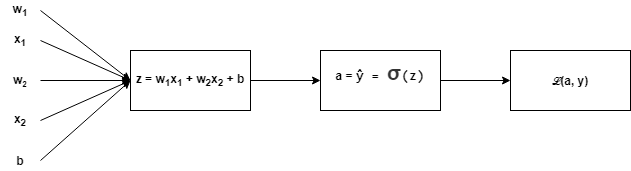
\includegraphics[scale=0.5]{books/artificial-neural-network/chapter02/figure/com_2.png}}
\caption{Sử dụng \textit{computation graph} vào \textit{logistic regression}}
\label{fig:com_2}
\end{figure}

Ta tính đạo hàm của $\mathcal{L}$ theo $a$ từ \ref{sec2:eqn28}:
\begin{equation}
\label{sec2:eqn31}
\frac{\partial \mathcal{L}}{\partial a} = -(y\frac{1}{a} + (1-y)\frac{-1}{1-a}) = \frac{1-y}{1-a} - \frac{y}{a} = \frac{a(1-y) - y(1-a)}{a(1-a)} = \frac{a-y}{a(1-a)}
\end{equation}

Sau đó, ta lan truyền kết quả lên để tính đạo hàm của $\mathcal{L}$ theo $z$ dựa trên đạo hàm của $\mathcal{L}$ theo $a$ từ \ref{sec2:eqn31} và đạo hàm của $a$ theo $z$:
\begin{align}
\frac{\partial a}{\partial z} &=  \frac{0(1 + e^{-z}) - (-e^{-z})1}{(1+e^{-z})^{2}} = \frac{e^{-z}}{(1+e^{-z})^{2}} = \frac{1}{1+e^{-z}\frac{e^{-z}}{1+e^{-z}}} = \frac{1}{1+e^{-z}}\frac{1+e^{-z}-1}{1+e^{-z}} = a(1-a)\\
\label{sec2:eqn33}
\frac{\partial \mathcal{L}}{\partial z} &= \frac{\partial \mathcal{L}}{\partial a}\frac{\partial a}{\partial z} = \frac{a-y}{a(1-a)}a(1-a) = a-y
\end{align}

Sau đó, ta lan truyền kết quả lên để tính đạo hàm của $\mathcal{L}$ theo $w_{1}$, $w_{2}$, $b$ dựa trên đạo hàm của $\mathcal{L}$ theo $z$ từ \ref{sec2:eqn33} và đạo hàm của $z$ theo $w_{1}$, $w_{2}$, $b$:
\begin{align}
\label{sec2:eqn34}
\frac{\partial z}{\partial w_{1}} &=  x_{1} \nonumber\\
\frac{\partial \mathcal{L}}{\partial w_{1}} &= \frac{\partial \mathcal{L}}{\partial z}\frac{\partial z}{\partial w_{1}} = (a-y)x_{1}\\
\label{sec2:eqn35}
\frac{\partial z}{\partial w_{2}} &=  x_{2} \nonumber\\
\frac{\partial \mathcal{L}}{\partial w_{2}} &= \frac{\partial \mathcal{L}}{\partial z}\frac{\partial z}{\partial w_{2}} = (a-y)x_{2}\\
\label{sec2:eqn36}
\frac{\partial z}{\partial b} &=  1 \nonumber\\
\frac{\partial \mathcal{L}}{\partial b} &= \frac{\partial \mathcal{L}}{\partial z}\frac{\partial z}{\partial b} = (a-y)
\end{align}

Suy ra, công thức \textit{computation graph} cho \textit{loss function} từ \ref{sec2:eqn34}, \ref{sec2:eqn35}, \ref{sec2:eqn36} là:
\begin{align}
\label{sec2:eqn37}
w_{1} = w_{1} - \alpha\frac{\partial \mathcal{L}}{\partial w_{1}} = w_{1} - \alpha(a-y)x_{1}\\
\label{sec2:eqn38}
w_{2} = w_{2} - \alpha\frac{\partial \mathcal{L}}{\partial w_{2}} = w_{2} - \alpha(a-y)x_{2}\\
\label{sec2:eqn39}
b = b - \alpha\frac{\partial \mathcal{L}}{\partial b} = b - \alpha(a-y)
\end{align}

\textit{Cost function} là tổng các \textit{loss funtion} của mỗi dữ liệu:
\begin{equation}
\label{sec2:eqn40}
J(w,b) = \frac{1}{m}\sum_{i=1}^{m}\mathcal{L}(a^{i}, x^{i})
\end{equation}

Từ đó, ta có thể tính được \textit{gradient decent} của \textit{cost function} bằng cách tính tổng \textit{gradient decent} các \textit{loss function} của dữ liệu từ \ref{sec2:eqn37}, \ref{sec2:eqn38}, \ref{sec2:eqn39}, \ref{sec2:eqn40}:
\begin{center}
$w_{1} = w_{1} - \alpha\frac{\partial J(w,b)}{\partial w_{1}} = w_{1} - \alpha\sum_{i=1}^m\frac{\partial \mathcal{L} (a^{i}, y^{i})}{\partial w_{1}} = w_{1} - \alpha\sum_{i=1}^m(a^{i} - y^{i})x_{1}^{i}$\\
$w_{2} = w_{2} - \alpha\frac{\partial J(w,b)}{\partial w_{2}} = w_{2} - \alpha\sum_{i=1}^m\frac{\partial \mathcal{L}(a^{i}, y^{i})}{\partial w_{2}} = w_{2} - \alpha\sum_{i=1}^m(a^{i} - y^{i})x_{2}^{i}$\\
$b = b - \alpha\frac{\partial J(w,b)}{\partial b} = b - \alpha\sum_{i=1}^m\frac{\partial \mathcal{L(a^{i}, y^{i})}}{\partial b} = b - \alpha\sum_{i=1}^m(a^{i} - y^{i})$
\end{center}

Một cách tổng quát hơn, với một dữ liệu gồm $n$ \textit{feature}, ta có \textit{gradient decent} là:
\begin{center}
$w_{1} =  w_{1} - \alpha\sum_{i=1}^m(a^{i} - y^{i})x_{1}^{i}$\\
$w_{2} =  w_{2} - \alpha\sum_{i=1}^m(a^{i} - y^{i})x_{2}^{i}$\\
\quad     \vdots\\
$w_{n} = w_{n} - \alpha\sum_{i=1}^m(a^{i} - y^{i})x_{n}^{i}$\\
$b =  b - \alpha\sum_{i=1}^m(a^{i} - y^{i})$
\end{center}

\section{Tổng kết phương pháp Logistic Regression}
Dưới đây là thuật giải của \textit{logistic regression} bằng mã giả:
\clearpage
\begin{algorithm}[!h]
\caption{Logistic regression}
$num\_iter=500, w1 = 0, w2 = 0, ..., wn = 0, b = 0, alpha = 0.1$\\
\For{ $i\gets1$ \KwTo $range(num_iter)$}{
    $J = 0, dw1 = 0, dw2 = 0, ..., dwn = 0, db = 0$\\
    \For{ $j\gets1$ \KwTo $m$}{
        $z = w1*xj1 + w2*xj2 + ... + wn*xjn + b$\\
        $a = 1/(1 + e^(-z))$\\
        $J += -(yj*log(aj) + (1 - yj)*log(1 - aj)$\\
        $dz = aj - yj$\\
        $dw1 += dz*xj1$\\
        $dw2 += dz*xj2$\\
        ...\\
        $dwn += dz*xjn$\\
        $db += dz$\\
    }
    $J/=m$\\
    $dw1/=m$\\
    $dw2/=m$\\
    ...\\
    $dwn/=m$\\
    $db/=m$\\
    $w1 = w1 - alpha*dw1$\\
    $w2 = w2 - alpha*dw2$\\
    ...\\
    $wn = wn - alpha*dwn$\\
    $b = b - alpha*b$
}
\end{algorithm}

Đoạn code trên là mã giả dùng để trình bày ý tưởng hiện thực \textit{logistic regression}. Ta xét trên một tập dữ liệu gồm $m$ dữ liệu và mỗi dữ liệu gồm $n$ \textit{feature}. Đầu tiên, chúng ta sẽ khai báo cáo biến cần thiết. Các $w1$, $w2$, ..., $wn$ lần lượt là các trọng số của mỗi \textit{feature} thuộc dữ liệu. $b$ là \textit{bias} được thêm vào. Giá trị num\_iter là số lần lặp để tìm được giá trị tối ưu của \textit{cost function}. Đây là giá trị ta có thể tuỳ chỉnh. Ta có thể gán 40, 50 hay 500 thâm chí đến 10000 tuỳ thuộc vào số lần lặp cần thiết để tìm được giá trị tối ưu của \textit{cost function}. $alpha$ là \textit{learning rate} mà ta thiết lập cho \textit{gradient decent}. Giá trị này không nên quá nhỏ hoặc quá lớn.

Tiếp theo, ta tính \textit{gradient decent} của \textit{cost function} bằng cách lặp lại việc cập nhật các trọng số với số lần lặp num\_iter cho trước.

Trong mỗi lần lặp, ta sẽ khởi tạo giá trị của \textit{cost function} $J$, các giá trị đạo hàm của $J$ theo $w1, w2, ..., wn$ là $dw1, dw2, ..., dwn$ và đạo hàm của $J$ theo $b$ là $wb$.

Ta sẽ chạy qua từng dữ liệu trong tập dữ liệu cho trước. Ta tính giá trị đầu ra. Tiếp đến, ta tính sự sai biệt giữa giá trị tính toán và giá trị thực tế dựa trên \textit{cross-entropy} và thêm kết quả vào \textit{cost function}. Sau khi chạy qua hết tập dữ liệu, ta tính giá trị đạo hàm của $J$ theo từng trọng số theo công thức được suy ra từ phần trước. Cuối cùng, ta cập nhật giá trị các trọng số dựa trên đạo hàm của chúng theo \textit{gradient decent}. Quá trình trên sẽ được lặp lại cho đến khi ta tìm được giá trị tối ưu của \textit{cost function} và thu được bộ trọng số thoả mãn yêu cầu.

\newpage
\section{Bài tập}
\begin{exer}
Từ dữ liệu của ví dụ \ref{exmp:o}, ta lấy một tập dữ liệu huấn luyện có kích thước m = 4, như bảng \ref{tab:exercise}:
\begin{table*}[ht]
\centering
\begin{tabular}{|l|l|l|l|}
\hline
Height & Gender \\ \hline
1.5   & F \\ \hline
1.75  & M \\ \hline
1.6     & M \\ \hline
1.45  & F  \\ \hline
\end{tabular}
\caption{Dữ liệu đầu vào của bài tập}
\label{tab:exercise}
\end{table*}

Sử dụng mô hình Logistic Regression $h\theta(x) = g(\theta_0 + \theta_1x_1)$ để giải bài toán phân loại Nam (M) và Nữ (F) dựa theo chiều cao của họ, với $x_1$ là vector chiều cao những người trong tập dữ liệu, $g$ là hàm sigmoid, và $\theta_0$, $\theta_1$ là hai trọng số cần phải học. Giả sử $y = 0$ khi một là nữ và $y = 1$ khi một người là nam, \textit{learning rate} $\alpha = 0.1$ và giá trị khởi tạo của $\theta_0$, $\theta_1$ là  $0$,  hàm mất mát là hàm \textit{Cross-Entropy}. Với tập dữ liệu training như bảng \ref{tab:exercise} và sử dụng mô hình Logistic Regression để cập nhật trọng số $\theta_0$ và $\theta_1$, hãy cho biết giá trị của hai trọng số $\theta_0$ và $\theta_1$ sau 2 lần lặp?
\end{exer}

\begin{exer}
Cho phương trình $J = a + 5(b + cd)$

Hãy vẽ computation graph của phương trình trên và tính đạo hàm của $J$ tại từng biến $a, b, c, d$ với $a=5, b=6, c=7, d=8$.
\end{exer}